\subsection{Zadania}

\begin{problem}
Niech $\set{G}\subseteq\set{F}$ będzie $\sigma$-ciałem. Rozważmy $\set{G}$-mierzalną zmienną losową $X$ oraz niezależną od $\set{G}$ zmienną losową $Y$. Załóżmy, że $\psi:\R^2\to\R$ jest taką funkcją mierzalną, że $\expected{|\psi(X, Y)|}<\infty$. Pokaż, że 
$$\expected{\psi(X, Y)}{\set{G}}=\Psi(X)\quad \Psi(x)=\expected{\psi(x, Y)}$$
\end{problem}

\begin{solution}
  Patrz dowód twierdzenia \ref{2.6 twierdzenie}.
\end{solution}

\begin{problem}
  Niech  $(X, Y)$ będzie dwuwymiarowym  wektorem losowych o rozkładzie jednostajnym na kwadracie o wierzchołkach $(-1, 0), (0, -1), (1, 0), (0, 1)$. Oblicz $\prob{X>\frac{1}{2}}{\set{Y}}$.
\end{problem}

\begin{solution}
  %Z definicji prawdopodobieństwa warunkowego mamy
  %$$\prob{X>\frac{1}{2}}{\set{Y}}=\expected{\mathds{1}_{\{X>1/2\}} }{\set{Y}}$$
  Zaczniemy od znalezienia gęstości rozkładu $X$ i $Y$.


  Oczywiście, gęstość rozkładu wektora $(X, Y)=\frac{1}{2}$ gdyż kwadrat ma pole $2$. W takim razie, gęstość zmiennej $X$ to 
  \begin{align*}
    f_X(x)&=\begin{cases}\int_{x-1}^{1-x}\frac{1}{2}dy  & x \geq 0\\ \int^{1+x}_{-x-1}\frac{1}{2}dy & x<0\end{cases}=\\ 
          &= \begin{cases}1-x & x\geq 0\\ 1+x&x<0\end{cases}
  \end{align*}
  W normalnych okolicznościach, prawdopodobieństwo, że $X>\frac{1}{2}$ wynosi
  $$\prob{X>\frac{1}{2}}=\int_{1/2}^1(1-x)dx=\frac{1}{8}$$

  \begin{center}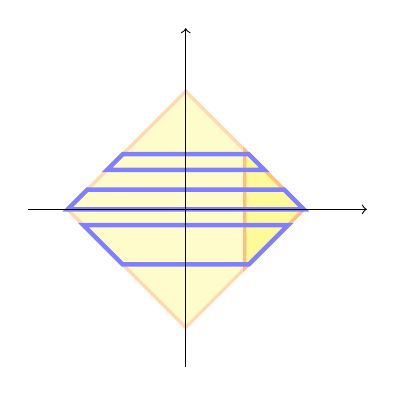
\begin{tikzpicture}
    \filldraw[color=orange!30, fill=yellow!20, very thick] (-1.5, 0)--(0, 1.5)--(1.5, 0)--(0, -1.5)--cycle;
    \filldraw[very thick, color=orange!50, fill=yellow!40] (1.5, 0)--(0.75, 0.75)--(0.75, -0.75)--cycle;
    \draw[color=blue!50, ultra thick] (-1.5, 0)--(1.5, 0)--(1.25, 0.25)--(-1.25, 0.25)--cycle;
    \draw[color=blue!50, ultra thick] (1, 0.5)--(-1, 0.5)--(-0.8, 0.7)--(0.8, 0.7)--cycle;
    \draw[color=blue!50, ultra thick] (-1.3, -0.2)--(1.3, -0.2)--(0.8, -0.7)--(-0.8, -0.7)--cycle;
    \draw[->] (0, -2)--(0, 2.3);
    \draw[->] (-2, 0)--(2.3, 0);
  \end{tikzpicture}\end{center}

  Niech $C\in\sigma(Y)$ takie, że $C=\{Y\in B\}$ dla $B\in Bor(\R)$ (niebieskie kształty na obrazku). Wtenczas
  \begin{align*}
    \expected{\prob{2X>1}{Y}\mathds{1}_C}&=\prob{\{2X>1\}\cap C}=\\ 
                                         &=\prob{\{2X>1\;i\;Y\in B\}}=\\ 
                                         &=\int_{B\cap [0, 1/2]}\int_{1/2}^{1-y}\frac{1}{2}dxdy+\int_{B\cap[-1/2, 0)}\int_{1/2}^{1+y}\frac{1}{2}dxdy=\\ 
                                         &=\frac{1}{2}\int_{B\cap [0, 1/2]}\left[\frac{1}{2}-y\right]dy+\frac{1}{2}\int_{B\cap[-1/2, 0)}\left[{\frac{1}{2}+y}\right]dy
  \end{align*}

  Czyli
  $$\prob{2X>1}{Y}=\frac{1}{2}\begin{cases}\frac{1}{2}-Y & Y\in[0, \frac{1}{2}]\\ \frac{1}{2}+Y & Y\in[-\frac{1}{2}, 0)\\ 0 & wpp.\end{cases}=h(Y),$$
  bo dla $C$ jak wyżej
  \begin{align*}
    \expected{h(Y)\mathds{1}_C}&=\expected{h(Y)\mathds{1}_{B\cap [0, 1/2]}}+\expected{h(Y)\mathds{1}_{B\cap[-1/2, 0)}}=\\ 
                               &=\frac{1}{2}\int_{B\cap [0, 1/2]}({1/2-y}) dy + \frac{1}{2}\int_{B\cap [-1, 0)}({1/2+y})dy
  \end{align*}

  [najmniej pewny fragment rozwiązania ahead]

  Próbując interpretować to geometrycznie, widać, że $2X>1$ tylko jeśli $Y\in[-1/2, 1/2]$. Dalej, jeśli ustalimy sobie jakiegoś dowolnego $Y$ z tego przedziału, to odległość od bliższego ogranicznika tego obszaru wynosi $\frac{1}{2}-Y$, jeśli $Y\geq 0$. Mnożąc to przez $2$ dostalibyśmy pole całego takiego paska: $[-1, 1]\times [Y, 1/2]$. Natomiast mnożąc przez $\frac{1}{2}$ dostajemy pole paska $[1/2, 1]\times[Y, 1/2]$.
  %stosunek długości kreski równoległej do $OX$ na wysokości tego $Y$ zachaczającej o $2X>1$ jest 1/4 długości całej kreski:
  \begin{center}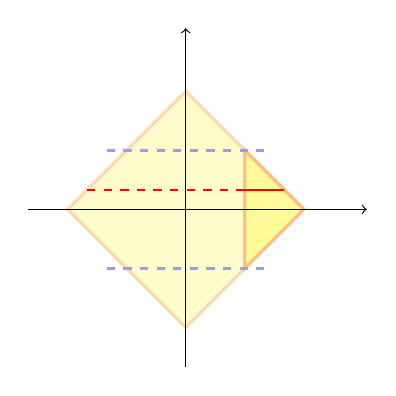
\begin{tikzpicture}
    \filldraw[color=orange!30, fill=yellow!20, very thick] (-1.5, 0)--(0, 1.5)--(1.5, 0)--(0, -1.5)--cycle;
    \filldraw[very thick, color=orange!50, fill=yellow!40] (1.5, 0)--(0.75, 0.75)--(0.75, -0.75)--cycle;
    \draw[->] (0, -2)--(0, 2.3);
    \draw[->] (-2, 0)--(2.3, 0);
    \draw[dashed, very thick, blue!40] (1, 0.75)--(-1, 0.75);
    \draw[dashed, very thick, blue!40] (1, -0.75)--(-1, -0.75);
    \draw[red, thick, dashed] (0.75, 0.25)--(-1.25, 0.25);
    \draw[red, thick] (1.25, 0.25)--(0.75, 0.25);
  \end{tikzpicture}\end{center}
  \end{solution}
